
\chapter{Concept Model}
\label{chap:lu.uni.lassy.excalibur.examples.icrash-CM}


\section{PrimaryTypes-Classes}
\subsection{Local view 01}
\label{sec:lu.uni.lassy.excalibur.examples.icrash-CM-view-local-PrimaryTypes-Classes-01}
Figure \ref{fig:lu.uni.lassy.excalibur.examples.icrash-CM-view-local-PrimaryTypes-Classes-01} 
shows the local view on all the primary types class types.



\begin{figure}[htbp] 
\label{fig:lu.uni.lassy.excalibur.examples.icrash-CM}
\begin{center}
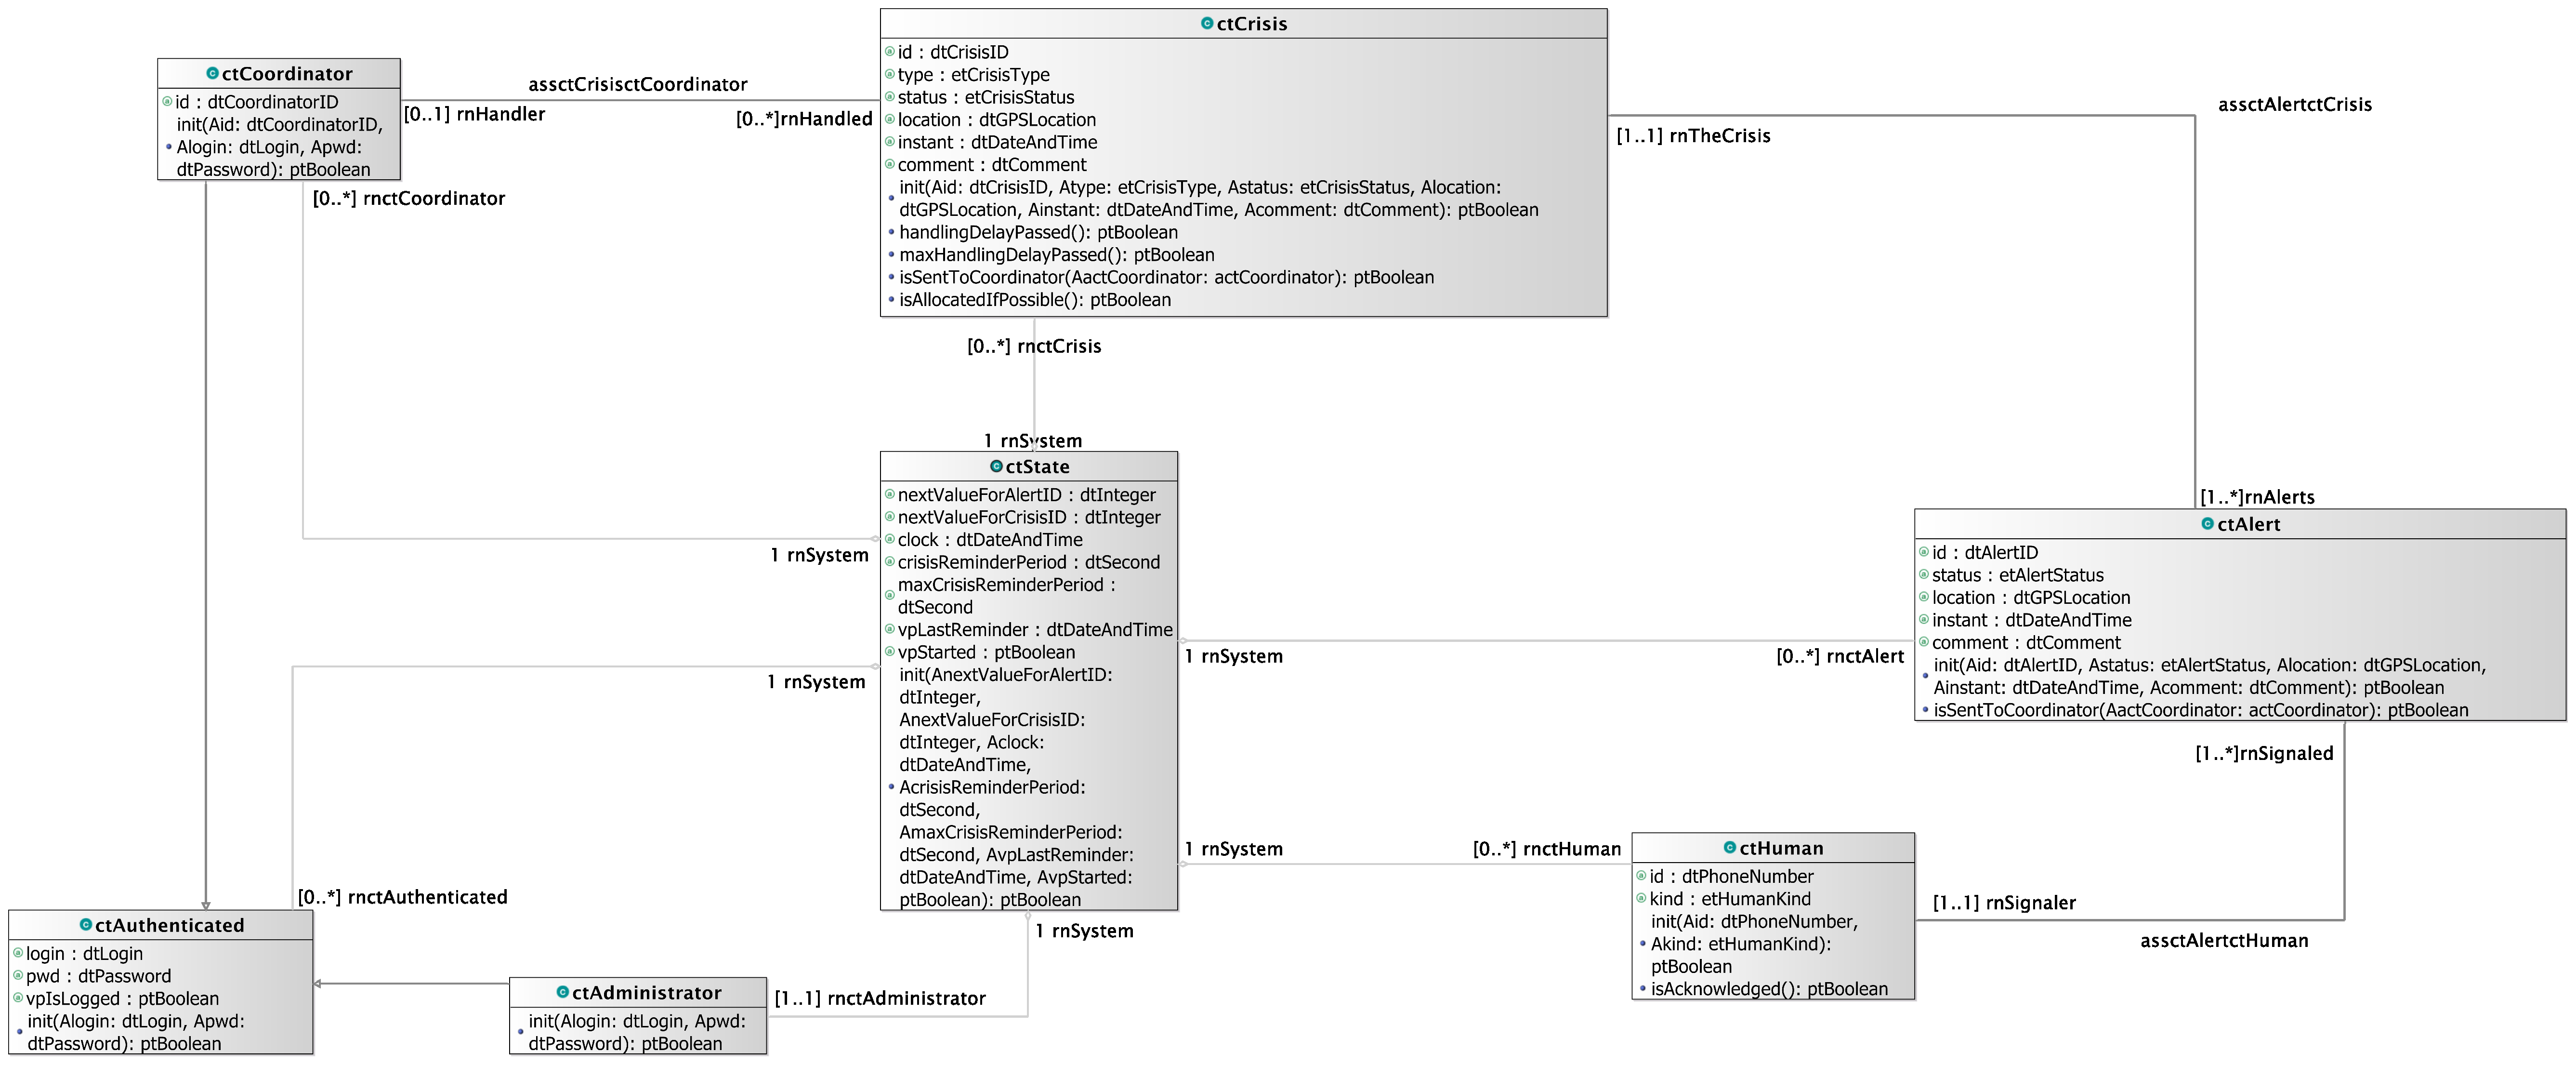
\includegraphics[
angle=0
,width=1.0\textwidth
]{./images-report-gen/concept-model/local/PrimaryTypes-Classes/01/cm-pt-ct-lv-01.eps}
\end{center}
\caption[Concept Model - PrimaryTypes-Classes local view 01 - Local view of all the primary types ]{Concept Model - PrimaryTypes-Classes local view 01. Local view of all the primary types class types
.}
\label{fig:lu.uni.lassy.excalibur.examples.icrash-CM-view-local-PrimaryTypes-Classes-01}
\end{figure}
\vspace{0.5cm} 

\subsection{Local view 02}
\label{sec:lu.uni.lassy.excalibur.examples.icrash-CM-view-local-PrimaryTypes-Classes-02}
Figure \ref{fig:lu.uni.lassy.excalibur.examples.icrash-CM-view-local-PrimaryTypes-Classes-02} shows the local view of the ctState primary type class type.



\begin{figure}[htbp] 
\label{fig:lu.uni.lassy.excalibur.examples.icrash-CM}
\begin{center}
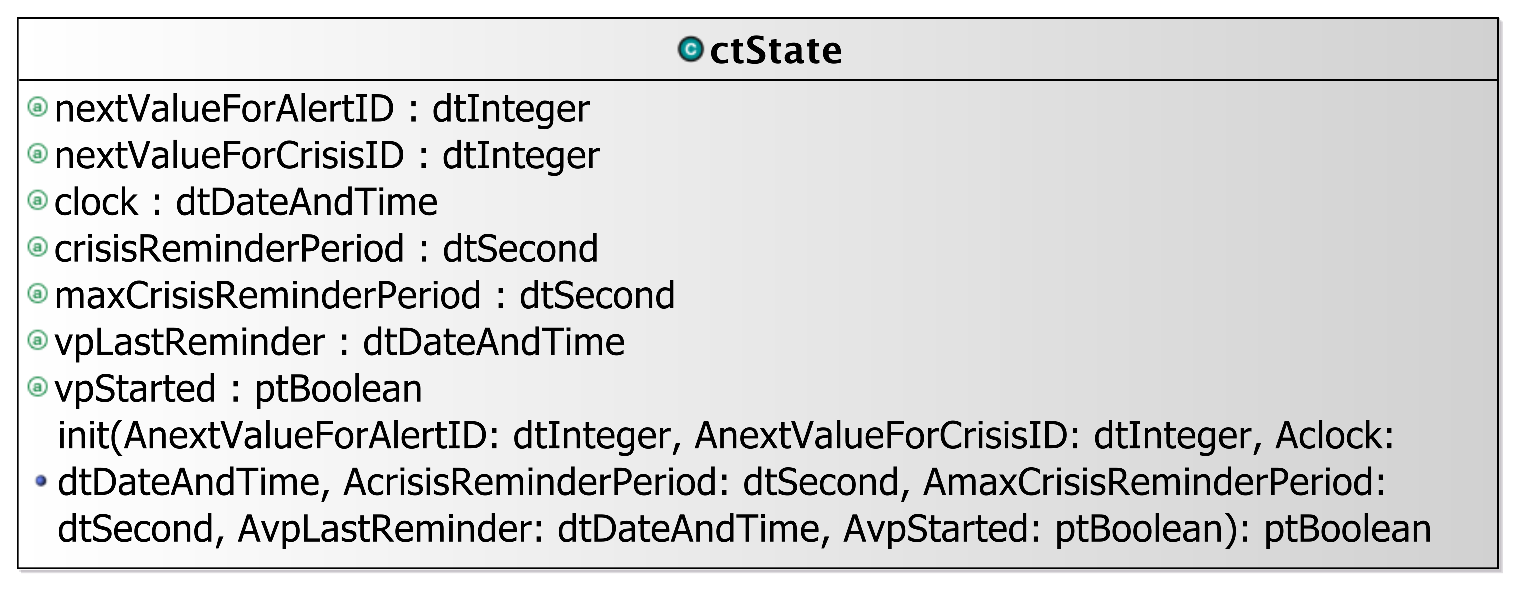
\includegraphics[
angle=0
,scale=0.80
]{./images-report-gen/concept-model/local/PrimaryTypes-Classes/02/cm-pt-ct-lv-02-parta-ctState.eps}
\end{center}
\caption[Concept Model - PrimaryTypes-Classes local view 02 - local view of the ctState primary ty]{Concept Model - PrimaryTypes-Classes local view 02. local view of the ctState primary type.}
\label{fig:lu.uni.lassy.excalibur.examples.icrash-CM-view-local-PrimaryTypes-Classes-02}
\end{figure}
\vspace{0.5cm} 

\subsection{Local view 03}
\label{sec:lu.uni.lassy.excalibur.examples.icrash-CM-view-local-PrimaryTypes-Classes-03}
Figure \ref{fig:lu.uni.lassy.excalibur.examples.icrash-CM-view-local-PrimaryTypes-Classes-03} shows the local view of the ctAlert primary type class type.



\begin{figure}[htbp] 
\label{fig:lu.uni.lassy.excalibur.examples.icrash-CM}
\begin{center}
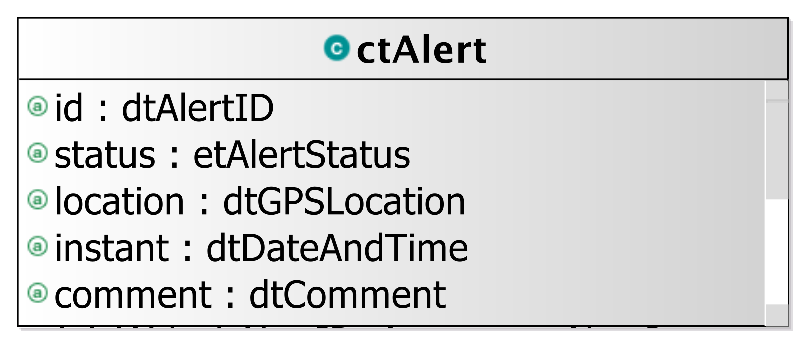
\includegraphics[
angle=0
,width=1.0\textwidth
]{./images-report-gen/concept-model/local/PrimaryTypes-Classes/03/cm-pt-ct-lv-03-partb-ctAlert.eps}
\end{center}
\caption[Concept Model - PrimaryTypes-Classes local view 03 - local view of the ctAlert primary ty]{Concept Model - PrimaryTypes-Classes local view 03. local view of the ctAlert primary type.}
\label{fig:lu.uni.lassy.excalibur.examples.icrash-CM-view-local-PrimaryTypes-Classes-03}
\end{figure}
\vspace{0.5cm} 

\subsection{Local view 04}
\label{sec:lu.uni.lassy.excalibur.examples.icrash-CM-view-local-PrimaryTypes-Classes-04}
Figure \ref{fig:lu.uni.lassy.excalibur.examples.icrash-CM-view-local-PrimaryTypes-Classes-04} shows the local view of the ctCrisis primary type class type.



\begin{figure}[htbp] 
\label{fig:lu.uni.lassy.excalibur.examples.icrash-CM}
\begin{center}
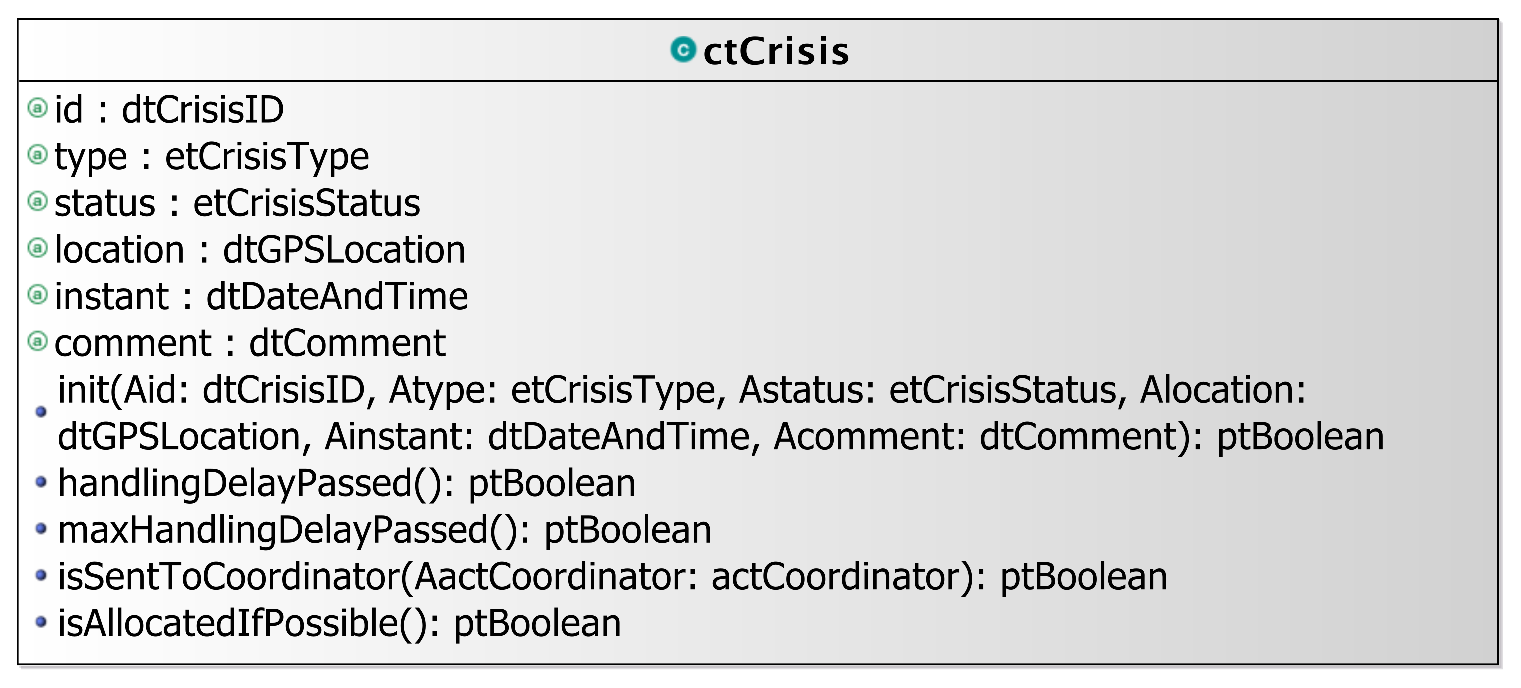
\includegraphics[
angle=0
,scale=0.80
]{./images-report-gen/concept-model/local/PrimaryTypes-Classes/04/cm-pt-ct-lv-04-partc-ctCrisis.eps}
\end{center}
\caption[Concept Model - PrimaryTypes-Classes local view 04 - local view of the ctCrisis primary t]{Concept Model - PrimaryTypes-Classes local view 04. local view of the ctCrisis primary type.}
\label{fig:lu.uni.lassy.excalibur.examples.icrash-CM-view-local-PrimaryTypes-Classes-04}
\end{figure}
\vspace{0.5cm} 


\subsection{Global view 01}
\label{sec:lu.uni.lassy.excalibur.examples.icrash-CM-view-global-PrimaryTypes-Classes-01}
Figure \ref{fig:lu.uni.lassy.excalibur.examples.icrash-CM-view-global-PrimaryTypes-Classes-01} 
shows the global view on primary types class types showing the association(s) types with the actor classes of the environment model.



\begin{figure}[htbp] 
\label{fig:lu.uni.lassy.excalibur.examples.icrash-CM}
\begin{center}
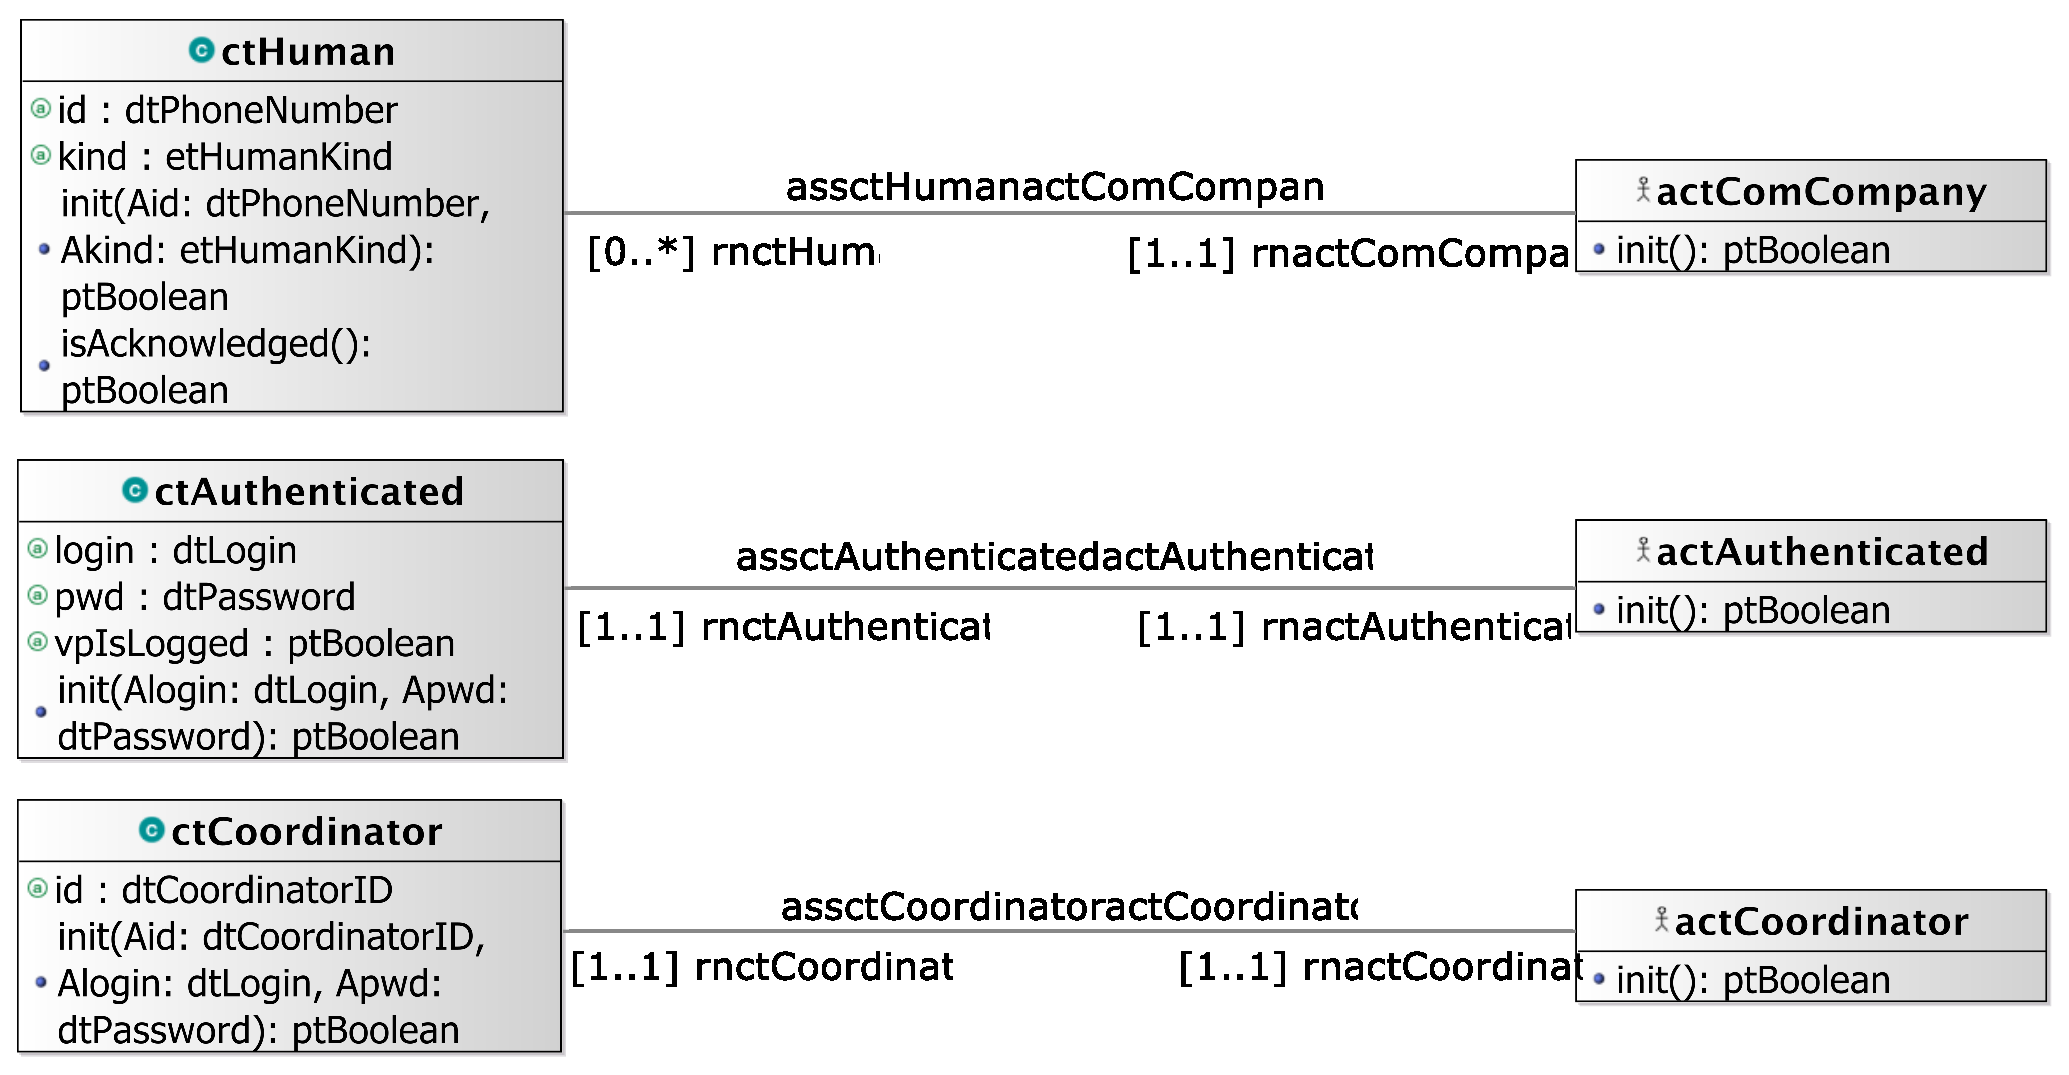
\includegraphics[
angle=0
,width=1.0\textwidth
]{./images-report-gen/concept-model/global/PrimaryTypes-Classes/01/cm-pt-ct-gv-01.eps}
\end{center}
\caption[Concept Model - PrimaryTypes-Classes global view 01 -  Primary types class types global vi]{Concept Model - PrimaryTypes-Classes global view 01.  Primary types class types global view - cm-pt-ct-gv-01
.}
\label{fig:lu.uni.lassy.excalibur.examples.icrash-CM-view-global-PrimaryTypes-Classes-01}
\end{figure}
\vspace{0.5cm} 



\section{PrimaryTypes-Datatypes}
\subsection{Local view 06}
\label{sec:lu.uni.lassy.excalibur.examples.icrash-CM-view-local-PrimaryTypes-Datatypes-06}
Figure \ref{fig:lu.uni.lassy.excalibur.examples.icrash-CM-view-local-PrimaryTypes-Datatypes-06} 



\begin{figure}[htbp] 
\label{fig:lu.uni.lassy.excalibur.examples.icrash-CM}
\begin{center}
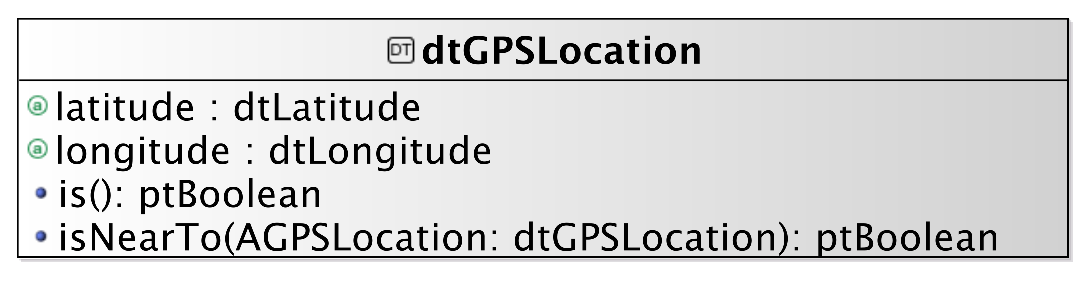
\includegraphics[
angle=0
]{./images-report-gen/concept-model/local/PrimaryTypes-Datatypes/06/cm-pt-dt-lv-02-dtGPSLocation.eps}
\end{center}
\caption[Concept Model - PrimaryTypes-Datatypes local view 06 - ]{Concept Model - PrimaryTypes-Datatypes local view 06. .}
\label{fig:lu.uni.lassy.excalibur.examples.icrash-CM-view-local-PrimaryTypes-Datatypes-06}
\end{figure}
\vspace{0.5cm} 


\subsection{Global view 01}
\label{sec:lu.uni.lassy.excalibur.examples.icrash-CM-view-global-PrimaryTypes-Datatypes-01}
Figure \ref{fig:lu.uni.lassy.excalibur.examples.icrash-CM-view-global-PrimaryTypes-Datatypes-01} 
shows a global view on the \msricrash primary types datatype types.



\begin{figure}[htbp] 
\label{fig:lu.uni.lassy.excalibur.examples.icrash-CM}
\begin{center}
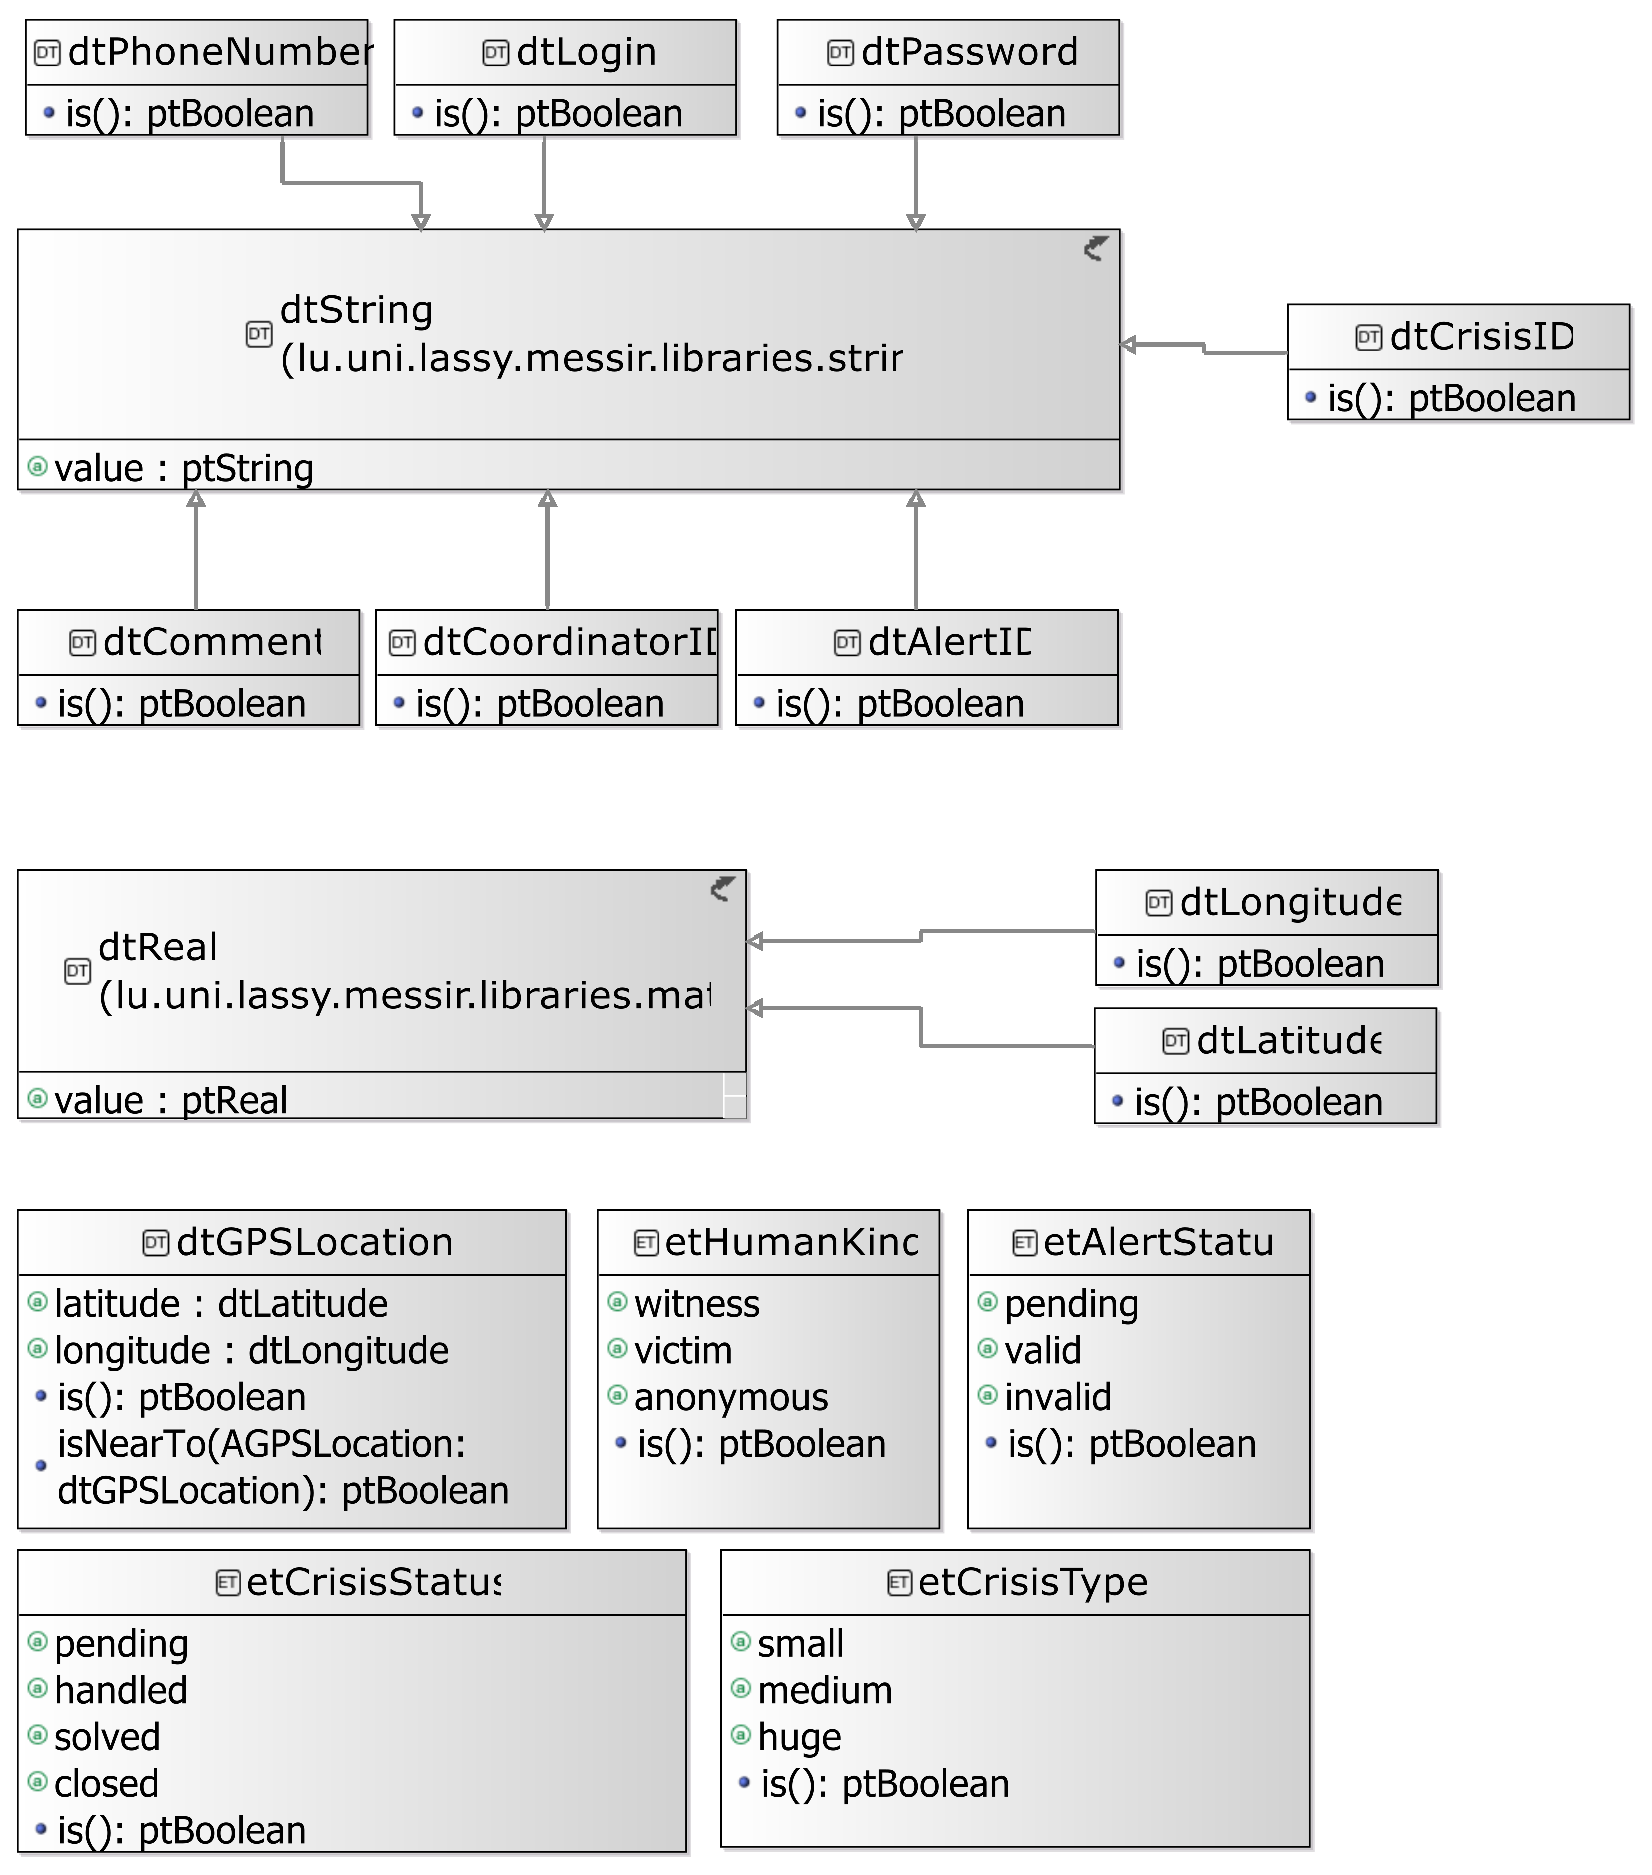
\includegraphics[
angle=0
,width=1.0\textwidth
]{./images-report-gen/concept-model/global/PrimaryTypes-Datatypes/01/cm-pt-dt-gv-01.eps}
\end{center}
\caption[Concept Model - PrimaryTypes-Datatypes global view 01 -  global view of primary types dataty]{Concept Model - PrimaryTypes-Datatypes global view 01.  global view of primary types datatype types - cm-pt-dt-gv-01
.}
\label{fig:lu.uni.lassy.excalibur.examples.icrash-CM-view-global-PrimaryTypes-Datatypes-01}
\end{figure}
\vspace{0.5cm} 





\section{SecondaryTypes-Datatypes}
\subsection{Local view 01}
\label{sec:lu.uni.lassy.excalibur.examples.icrash-CM-view-local-SecondaryTypes-Datatypes-01}
Figure \ref{fig:lu.uni.lassy.excalibur.examples.icrash-CM-view-local-SecondaryTypes-Datatypes-01} shows the local view of the secondary types datatype types.



\begin{figure}[htbp] 
\label{fig:lu.uni.lassy.excalibur.examples.icrash-CM}
\begin{center}
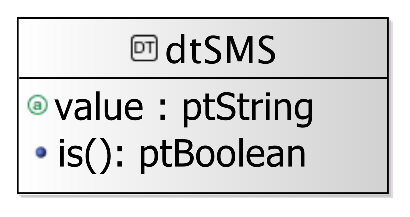
\includegraphics[
angle=0
]{./images-report-gen/concept-model/local/SecondaryTypes-Datatypes/01/cm-st-dt-lv-01.eps}
\end{center}
\caption[Concept Model - SecondaryTypes-Datatypes local view 01 - Local view of the secondary types da]{Concept Model - SecondaryTypes-Datatypes local view 01. Local view of the secondary types datatype types.}
\label{fig:lu.uni.lassy.excalibur.examples.icrash-CM-view-local-SecondaryTypes-Datatypes-01}
\end{figure}
\vspace{0.5cm} 






\section{Concept Model Types Descriptions}
This section provides the textual descriptions of all the types defined in the concept model and that can be part of the graphical views provided.

\subsection{Primary types - Class types descriptions}




The table below is providing comments on the graphical views given for the class types of the primary types. Type logical operations are precisely specified in the operation model.

\begin{datadictionary}
\addheading{Classes}

\adddoublerow{ctAdministrator}{used to caracterize internally the entity that is responsible of administrating the \msricrash system.}
\addsingletwocolumnrow{extends}{icrash.concepts.primarytypes.classes.ctAuthenticated}
\adddoubletwocolumnrow{operation}{\msrcode{init(Alogin:dtLogin, Apwd:dtPassword):ptBoolean}}{used to initialize the current object as a new instance of the ctAdministrator type.}
\adddoublerow{ctAlert}{Used to model crisis alerts sent by any human having communication capability using communication companies belonging to the system's environment}
\adddoubletwocolumnrow{attribute}{\msrcode{comment: dtComment}}{a textual description providing unstructured information on the alert.}
\adddoubletwocolumnrow{attribute}{\msrcode{id: dtAlertID}}{the alert unique identification information.}
\adddoubletwocolumnrow{attribute}{\msrcode{instant: dtDateAndTime}}{the date and time at which the alert notification has been sent.}
\adddoubletwocolumnrow{attribute}{\msrcode{location: dtGPSLocation}}{the position of the alert provided by the space-based satellite navigation system used by the human using the communication company to inform the \msricrash system of a crisis.}
\adddoubletwocolumnrow{attribute}{\msrcode{status: etAlertStatus}}{the alert validation status }
\adddoubletwocolumnrow{operation}{\msrcode{init(Aid:dtAlertID, Astatus:etAlertStatus, Alocation:dtGPSLocation, Ainstant:dtDateAndTime, Acomment:dtComment):ptBoolean}}{used to initialize the current object as a new instance of the ctAlert type.}
\adddoubletwocolumnrow{operation}{\msrcode{isSentToCoordinator(AactCoordinator:actCoordinator):ptBoolean}}{used to provide a given coordinator with current alert information.}
\adddoublerow{ctAuthenticated}{used to model system's representation about actors that need to authenticate to access some specific functionalities.}
\adddoubletwocolumnrow{attribute}{\msrcode{login: dtLogin}}{an identifier for authentication.}
\adddoubletwocolumnrow{attribute}{\msrcode{pwd: dtPassword}}{a key for authentication.}
\adddoubletwocolumnrow{attribute}{\msrcode{vpIsLogged: ptBoolean}}{used to determine the access status.}
\adddoubletwocolumnrow{operation}{\msrcode{init(Alogin:dtLogin, Apwd:dtPassword):ptBoolean}}{used to initialize the current object as a new instance of the ctAuthenticated type.}
\adddoublerow{ctCoordinator}{used to model system's representation about the actors that have the responsibility to handle alerts and crisis.}
\addsingletwocolumnrow{extends}{icrash.concepts.primarytypes.classes.ctAuthenticated}
\adddoubletwocolumnrow{attribute}{\msrcode{id: dtCoordinatorID}}{a unique identification information.}
\adddoubletwocolumnrow{operation}{\msrcode{init(Aid:dtCoordinatorID, Alogin:dtLogin, Apwd:dtPassword):ptBoolean}}{used to initialize the current object as a new instance of the ctCoordinator type.}
\adddoublerow{ctCrisis}{Used to model crisis that are infered from the reception of at least one alert message. Crisis aer entities that are handled by the \msricrash system.}
\adddoubletwocolumnrow{attribute}{\msrcode{comment: dtComment}}{a textual description providing unstructured information on the crisis handling.}
\adddoubletwocolumnrow{attribute}{\msrcode{id: dtCrisisID}}{the crisis unique identification information.}
\adddoubletwocolumnrow{attribute}{\msrcode{instant: dtDateAndTime}}{the date and time at which the first related alert notification has been sent.}
\adddoubletwocolumnrow{attribute}{\msrcode{location: dtGPSLocation}}{the position of the crisis equal by the one of the first alert received and associated to the crisis.}
\adddoubletwocolumnrow{attribute}{\msrcode{status: etCrisisStatus}}{the crisis handling status.}
\adddoubletwocolumnrow{attribute}{\msrcode{type: etCrisisType}}{an indication of the gravity of the crisis.}
\adddoubletwocolumnrow{operation}{\msrcode{handlingDelayPassed():ptBoolean}}{used to determine if the crisis stood too longly in a pending status since last reminder.}
\adddoubletwocolumnrow{operation}{\msrcode{init(Aid:dtCrisisID, Atype:etCrisisType, Astatus:etCrisisStatus, Alocation:dtGPSLocation, Ainstant:dtDateAndTime, Acomment:dtComment):ptBoolean}}{used to initialize the current object as a new instance of the ctAlert type.}
\adddoubletwocolumnrow{operation}{\msrcode{isAllocatedIfPossible():ptBoolean}}{used to allocate a crisis to a coordinator if any or to alert the administrator of crisis waiting to be handled.}
\adddoubletwocolumnrow{operation}{\msrcode{isSentToCoordinator(AactCoordinator:actCoordinator):ptBoolean}}{used to provide a given coordinator with current crisis information.}
\adddoubletwocolumnrow{operation}{\msrcode{maxHandlingDelayPassed():ptBoolean}}{used to determine if the crisis stood too longly in a pending status since its creation.}
\adddoublerow{ctHuman}{used to model system's representation about the indirect actors that has alerted of potential crisis.}
\adddoubletwocolumnrow{attribute}{\msrcode{id: dtPhoneNumber}}{the number of the communication device used to send an alert to \msricrash system.}
\adddoubletwocolumnrow{attribute}{\msrcode{kind: etHumanKind}}{role with respect to the alert notified.}
\adddoubletwocolumnrow{operation}{\msrcode{init(Aid:dtPhoneNumber, Akind:etHumanKind):ptBoolean}}{\msrcode{init}: used to initialize the current object as a new instance of the ctHuman type.}
\adddoublerow{ctState}{used to model the system. Each system specified using \msrmessir must include a ctState class for which there is only one instance at any state of the abstract machine after creation.}
\adddoubletwocolumnrow{attribute}{\msrcode{clock: dtDateAndTime}}{used to represent the system local time.}
\adddoubletwocolumnrow{attribute}{\msrcode{crisisReminderPeriod: dtSecond}}{used to define the delay between two reminders after which a reminder must be sent to the administrator and to the known coordinators to encourage them to handle the crisis.}
\adddoubletwocolumnrow{attribute}{\msrcode{maxCrisisReminderPeriod: dtSecond}}{used to define the maximum delay after which the crisis is ramdomly allocated to a coordinator if any or an alert message is sent to the administrator in order to encourage him to add coordinators.}
\adddoubletwocolumnrow{attribute}{\msrcode{nextValueForAlertID: dtInteger}}{\msrcode{nextValueForAlertID: dtInteger}: used to associate each alert declared with a unique idenitification value. }
\adddoubletwocolumnrow{attribute}{\msrcode{nextValueForCrisisID: dtInteger}}{used to associate each crisis declared with a unique idenitification value. }
\adddoubletwocolumnrow{attribute}{\msrcode{vpLastReminder: dtDateAndTime}}{date and time of the last reminder.}
\adddoubletwocolumnrow{attribute}{\msrcode{vpStarted: ptBoolean}}{used to avoid reacting to an actor message if the system is not started (i.e. oeCreateSystemAndEnvironment not executed).}
\adddoubletwocolumnrow{operation}{\msrcode{init(AnextValueForAlertID:dtInteger, AnextValueForCrisisID:dtInteger, Aclock:dtDateAndTime, AcrisisReminderPeriod:dtSecond, AmaxCrisisReminderPeriod:dtSecond, AvpLastReminder:dtDateAndTime, AvpStarted:ptBoolean):ptBoolean}}{used to initialize the current object as a new instance of the ctState type.}
\end{datadictionary}

\subsection{Primary types - Datatypes types descriptions}



There are no elements in this category in the system analysed.



\subsection{Primary types - Association types descriptions}




The table below is providing comments on the association types of the primary types.

\begin{associationtypes}
\addheading{Undirected associations}
\adddoublerow{assctAlertctCrisis}{a crisis is related to one or more alerts as the alerts judged to concern all the same crisis due to their location. An alert alerts exactly one crisis.}
\adddoublerow{assctAlertctHuman}{ alerts are notified by human through the communication company. We need to keep an internal representation of those human to allow for communication of alert handling.}
\adddoublerow{assctAuthenticatedactAuthenticated}{mainly used to determine if the login request of an authenticated actor can be granted based on the given credentials and the registered ones.}
\adddoublerow{assctCoordinatoractCoordinator}{frequent messages must be sent to coordinator especially in relation to crisis they handle.}
\adddoublerow{assctCrisisctCoordinator}{at any point in time we need to know if a coordinator is handling existing crisis or not.}
\adddoublerow{assctHumanactComCompany}{ in order to communicate with humans who informed about potential crisis, we need to record the communication company to use to send them messages.}
\end{associationtypes}

\subsection{Primary types - Aggregation types descriptions}


There are no aggregation types for the primary types.


\subsubsection{Primary types - Composition types descriptions}



There are no composition types for the primary types.


\subsection{Secondary types - Class types descriptions}



There are no elements in this category in the system analysed.
		

\subsection{Secondary types - Datatypes types descriptions}





The table below is providing comments on the graphical views given for the datatype types of the secondary types.

\begin{datadictionary}
\addheading{Datatypes}

\adddoublerow{dtSMS}{a datatype made of a string value used to send textual information to human mobile devices.}
\adddoubletwocolumnrow{attribute}{\msrcode{value: ptString}}{the textual information.}
\adddoubletwocolumnrow{operation}{\msrcode{is():ptBoolean}}{used to determine which strings are considered as valid comments.}
\end{datadictionary}





\subsection{Secondary types - Association types descriptions}



There are no association types for the secondary types.



\subsection{Secondary types - Aggregation types descriptions}



There are no aggregation types for the secondary types.



\subsection{Secondary types - Composition types descriptions}



There are no composition types for the secondary types.



